\section{Solving Linear Equations}
    
    \subsection{Vectors and Linear Equations}
        Given a set of two linear equations,
        \begin{equation}
            \begin{split}
                x - 2y &= 1 \\
                3x + 2y &= 11
            \end{split}
        \end{equation}
        finding the solution to \(x\) and \(y\) in the usual \textbf{row form} involves finding the point at which the two lines intersect, as seen in the figure below.
        \begin{figure}[h]
            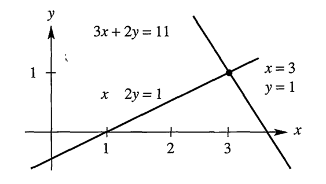
\includegraphics[width=0.50\textwidth]{vectors_and_linear_equations_0}
            \centering
            \caption{Solution to two linear equation using the row method}
        \end{figure}
        \par \hfill \break
        Expressing this in \textbf{column form}, being the linear combination of the vectors, using the solutions found
        for the row form, results in the output vector \(\boldsymbol{b}\). However, the problem here is to find the 
        values of the coefficients \(x\) and \(y\).
        \begin{figure}[h]
            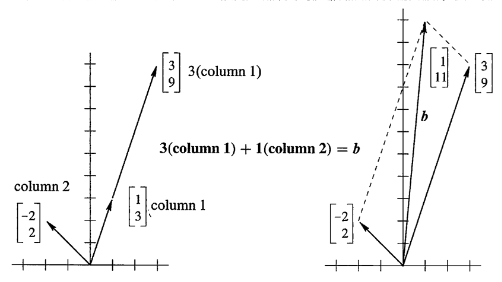
\includegraphics[width=0.50\textwidth]{vectors_and_linear_equations_1}
            \centering
            \caption{Column form}
        \end{figure}

        \subsubsection{Three Equations in Three Unknowns}
            The same can be applied to three equations in three unknowns,
            \begin{equation}
                \begin{split}
                    x + 2y +3z &= 6 \\
                    2x + 5y + 2z &= 4 \\
                    6x - 3y + z &= 2
                \end{split}
            \end{equation}
            However this time each row forms a \textbf{plane} in three-dimensional space. The \textbf{row picture} is then seen as,
            \begin{figure}[h]
                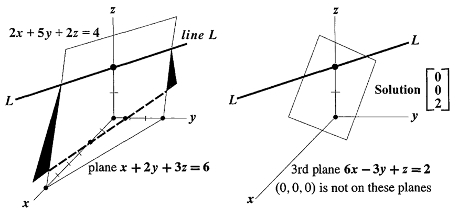
\includegraphics[width=0.50\textwidth]{vectors_and_linear_equations_2}
                \centering
                \caption{Solution to two linear equation using the row method}
            \end{figure}
            \par \hfill \break
            and the \textbf{column picture}, once the \(x\), \(y\) and \(z\) coefficients area found, is then seen as,
            \begin{figure}[h]
                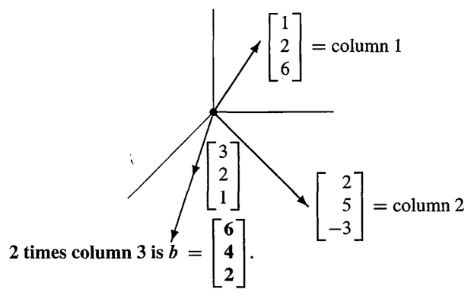
\includegraphics[width=0.50\textwidth]{vectors_and_linear_equations_3}
                \centering
                \caption{Solution to two linear equation using the column method}
            \end{figure}

    \subsection{The Idea of Elimination}
        The basic idea of elimination is the to reduce the equation coefficients and produce an 
        \textbf{upper triangular matrix}, then using a process called \textbf{back substitution}, to solve for \(x\) and
        \(y\). An example being,
        \begin{equation}
            \begin{split}
                x - 2y &= 1 \\
                3x + 2y &= 11
            \end{split}
            \quad \rightarrow \quad
            \begin{split}
                x - 2y &= 1 \\
                8y &= 8
            \end{split}
        \end{equation}
        Here, the first equation is multiplied by 3 and subtracted from the second. This results in \(y = 1\), 
        inserting this into the first equation yeilds \(x = 3\). 
        \par \hfill \break
        A \textbf{pivot is the first non-zero element in the row that does the elimination}, so 1 in this case, and the 
        \textbf{multiplier is the value for which the equation of the pivot is multiplied by}, so 3. The next pivots are
        then diagonal entries in the matrix of coefficients, which in this case would be 8.
        \par \hfill \break
        Pivots cannot be zero, and if a pivot is zero then this results in no solution, or an infinite number of 
        solutions, and a \textbf{singular matrix}. When there is a full set of pivots and exactly one solution, 
        the matrix is \textbf{non-singular}.

    \subsection{Elimination using Matrices}
        As seen in the last section, elimination is the process of the producing an upper triangular matrix with which
        a solution may be found by then performing back substitution. This was generally performed a row at a time, but
        can also be performed using an elimination matrix \(E_{ij}\), so the form of the equation
        \(A\boldsymbol{x} = \boldsymbol{b}\), is then expressed as \(E(A\boldsymbol{x}) = E(\boldsymbol{b})\).
        \par \hfill \break
        Considering example in the previous section, the matrix form would look as follows,
        \begin{equation}
            \begin{bmatrix}
                1 & -2 \\
                3 & 2
            \end{bmatrix}
            \begin{bmatrix}
                x \\
                y
            \end{bmatrix}
            =
            \begin{bmatrix}
                1 \\
                11
            \end{bmatrix}
            \quad \rightarrow \quad
            \begin{bmatrix}
                1 & -2 \\
                0 & 8
            \end{bmatrix}
            \begin{bmatrix}
                x \\
                y
            \end{bmatrix}
            =
            \begin{bmatrix}
                1 \\
                8
            \end{bmatrix}
        \end{equation}
        Multiplcation of the elimination matrix would result in,
        \begin{equation}
            \begin{bmatrix}
                1 & 0 \\
                -3 & 1
            \end{bmatrix}
            \begin{bmatrix}
                1 & -2 \\
                3 & 2
            \end{bmatrix}
            \begin{bmatrix}
                x \\
                y
            \end{bmatrix}
            =
            \begin{bmatrix}
                1 & 0 \\
                -3 & 1
            \end{bmatrix}
            \begin{bmatrix}
                1 \\
                11
            \end{bmatrix}
            \quad \rightarrow \quad
            \begin{bmatrix}
                1 & -2 \\
                0 & 8
            \end{bmatrix}
            \begin{bmatrix}
                x \\
                y
            \end{bmatrix}
            =
            \begin{bmatrix}
                1 \\
                8
            \end{bmatrix}
        \end{equation}
        \par \hfill \break
        When performing matrix multiplication, the expression of 
        \(\boldsymbol{E}(\boldsymbol{Ax}) = \boldsymbol{E}(\boldsymbol{b})\) can also be written as 
        \((\boldsymbol{EA})\boldsymbol{x} = \boldsymbol{E}(\boldsymbol{b})\) given the associative law which states
        \(\boldsymbol{A}(\boldsymbol{BC})=(\boldsymbol{AB})\boldsymbol{C}\). It should be noted that the commutative 
        law is does not apply, so \(\boldsymbol{AB} \neq \boldsymbol{BA}\) in general.

        \subsubsection{Permutation Matrix}
            Similar to the elimination matrix, a \textbf{permutation matrix} has the action of swapping rows the of 
            matrix it acts on. An example permutation matrix which has the action of swapping the 2\textsuperscript{nd}
            and 3\textsuperscript{rd} rows of a matrix is seen below,
            \begin{equation}
                P_{ij} = 
                \begin{bmatrix}
                    1 & 0 & 0 \\
                    0 & 0 & 1 \\
                    0 & 1 & 0 
                \end{bmatrix}
            \end{equation}
        
        \subsubsection{Augmented Matrix}
            The form of the elimination equation \(EA\boldsymbol{x}=E\boldsymbol{b}\) has the elimination equation 
            acting on both the \(A\) and \(\boldsymbol{b}\) parts of the equation separately. By expressing the vector
            \(\boldsymbol{b}\) on the same side as the coefficient matrix \(A\), the elimination matrix may then act on the
            full expression of \([A \boldsymbol{b}]\). This form is known as the \textbf{augmented matrix}.
            \par \hfill \break
            For example, given the equation,
            \begin{equation}
                \begin{bmatrix}
                    2 & 4 & -2 \\
                    4 & 9 & -3 \\
                    -2 & -3 & 7 
                \end{bmatrix}
                \begin{bmatrix}
                    x \\
                    y \\
                    z
                \end{bmatrix}
                =
                \begin{bmatrix}
                    2 \\
                    8 \\
                    10
                \end{bmatrix}
            \end{equation}
            The augmented matrix would be,
            \begin{equation}
                Aug_{ij} = 
                \begin{bmatrix}
                    2 & 4 & -2 & \boldsymbol{2} \\
                    4 & 9 & -3 & \boldsymbol{8} \\
                    -2 & -3 & 7 & \boldsymbol{10}
                \end{bmatrix}
            \end{equation}
            Multiplication may then be performed on the whole matrix, such as in combination with the elimination 
            matrix, \(E[A\boldsymbol{b}]\).

    \subsection{Rules for Matrix Operations}

        \subsubsection{Matrix Multiplication}

            \textbf{Inner (Dot) Product}
            \par \hfill \break
            The classical way of multiplying matrices is by using the \textbf{inner product}, also known as the
            \textbf{dot product}. In terms of multiplication of matrices \(A\) and \(B\), this works by finding the dot
            product of each of the rows of \(A\) and respective columns of \(B\),
            
            \par \hfill \break
            \textbf{Rows and Columns}
            \par \hfill \break
            The next two methods consider multiplication of the rows and columns with a matrix.
            \par \hfill \break
            The \textbf{row form} multiplies the matrix \(A\) with a row of \(b\) vectors, with each vector being a
            column of \(b\),
            \begin{equation}
                AB = A
                \begin{bmatrix}
                    \boldsymbol{b}_1 & ... & \boldsymbol{b}_m
                \end{bmatrix}
                =
                \begin{bmatrix}
                    A\boldsymbol{b}_1 & ... & A\boldsymbol{b}_m
                \end{bmatrix}
            \end{equation}
            An example being, 
            \begin{equation}
                \begin{bmatrix}
                    1 & 1 \\
                    2 & -1
                \end{bmatrix}
                \begin{bmatrix}
                    2 & 2 \\
                    3 & 4
                \end{bmatrix}
                =
                \begin{bmatrix}
                    \begin{bmatrix}
                        1 & 1 \\
                        2 & -1
                    \end{bmatrix}
                    \begin{bmatrix}
                        2 \\
                        3
                    \end{bmatrix}
                    &
                    \begin{bmatrix}
                        1 & 1 \\
                        2 & -1
                    \end{bmatrix}
                    \begin{bmatrix}
                        2 \\
                        3
                    \end{bmatrix}
                \end{bmatrix}
                =
                \begin{bmatrix}
                    5 & 6 \\
                    1 & 0
                \end{bmatrix}
            \end{equation}
            The \textbf{column form} multiplies a column vector consisting of the rows of \(a\) with the matrix \(B\).
            \begin{equation}
                AB =
                \begin{bmatrix}
                    \boldsymbol{a}_1 \\
                    ... \\
                    \boldsymbol{a}_m
                \end{bmatrix}
                B
                =
                \begin{bmatrix}
                    \boldsymbol{a}_1 B\\
                    ... \\
                    \boldsymbol{a}_m B
                \end{bmatrix}
            \end{equation}
            An example being, 
            \begin{equation}
                \begin{bmatrix}
                    1 & 1 \\
                    2 & -1
                \end{bmatrix}
                \begin{bmatrix}
                    2 & 2 \\
                    3 & 4
                \end{bmatrix}
                =
                \begin{bmatrix}
                    \begin{bmatrix}
                        1 & 1
                    \end{bmatrix}
                    \begin{bmatrix}
                        2 & 2 \\
                        3 & 4
                    \end{bmatrix} \\
                    \begin{bmatrix}
                        2 & -1
                    \end{bmatrix}
                    \begin{bmatrix}
                        2 & 2 \\
                        3 & 4
                    \end{bmatrix}
                \end{bmatrix}
                =
                \begin{bmatrix}
                    5 & 6 \\
                    1 & 0
                \end{bmatrix}
            \end{equation}
            
            \par \hfill \break
            \textbf{Columns Multiply Rows}
            \par \hfill \break
            The last method involves multiplication of the columns of matrix \(A\) by the rows of \(B\), then summing
            the individual matrices to the result. So,
            \begin{equation}
                AB =
                \begin{bmatrix}
                    \boldsymbol{a}_1 & ... & \boldsymbol{a}_m
                \end{bmatrix}
                \begin{bmatrix}
                    \boldsymbol{b}_1 \\
                    ... \\
                    \boldsymbol{b}_n
                \end{bmatrix}
                =
                \begin{bmatrix}
                    \boldsymbol{a}_1 \boldsymbol{b}_1 & ... & \boldsymbol{a}_m \boldsymbol{b}_n
                \end{bmatrix}
            \end{equation}
            As an example,
            \begin{equation}
                \begin{bmatrix}
                    1 & 1 \\
                    2 & -1
                \end{bmatrix}
                \begin{bmatrix}
                    2 & 2 \\
                    3 & 4
                \end{bmatrix}
                =
                \begin{bmatrix}
                    1 \\
                    2
                \end{bmatrix}
                \begin{bmatrix}
                    2 & 2
                \end{bmatrix}
                +
                \begin{bmatrix}
                    1 \\
                    -1
                \end{bmatrix}
                \begin{bmatrix}
                    3 & 4
                \end{bmatrix}
                =
                \begin{bmatrix}
                    5 & 6 \\
                    1 & 0
                \end{bmatrix}
            \end{equation}
        
        \subsubsection{Matrix Operation Laws}
        
            \par \hfill \break
            \textbf{Addition / Subtraction}
            \par \hfill \break
            The laws for addition and subtraction covers the \textbf{commutative} law which states that 
            \begin{equation}
                A + B = B + A
            \end{equation}
            the \textbf{distributive} law which states that 
            \begin{equation}
                c(A + B) = cA + cB
            \end{equation}
            and the \textbf{associative} law which states that 
            \begin{equation}
                A+(B+C) = (A+B)+C
            \end{equation}.

            \par \hfill \break
            \textbf{Multiplication}
            \par \hfill \break
            The laws for multiplication cover the \textbf{commutative} law which states that 
            \begin{equation}
                AB \neq BA
            \end{equation}
            the \textbf{distributive from left} law which states that 
            \begin{equation}
                A(B+C)=AB+AC
            \end{equation}
            the \textbf{distributive from right} law which states that 
            \begin{equation}
                (A+B)C=AC+BC
            \end{equation}
            and the \textbf{associative} law which states that 
            \begin{equation}
                A(BC) = A(BC)
            \end{equation}

            \par \hfill \break
            \textbf{Factors}
            \par \hfill \break
            The factors law states that 
            \begin{equation}
                A^p = AA ... A \quad  \textrm{for all \(p\)}
            \end{equation}
            and 
            \begin{equation}
                A^p A^q = A^{p+q}
            \end{equation}

        \subsubsection{Block Matrices}
            A matrix may be split into smaller matrix blocks and analysed that way for simplicity. In this way, a      
            larger matrix \(A\) and \(B\) are split into smaller matrices, \(A_11\), \(A_12\), etc and \(B_11\), 
            \(B_21\) and then applying matric multiplication as usual.
            \begin{equation}
                \begin{bmatrix}
                    A_{11} & A_{12} \\
                    A_{21} & A_{22}
                \end{bmatrix}
                \begin{bmatrix}
                    B_{11} \\
                    B_{21}
                \end{bmatrix}
                =
                \begin{bmatrix}
                    A_{11} B_{11} & A_{12} B_{21} \\
                    A_{21} B_{11} & A_{22} B_{21}
                \end{bmatrix}
            \end{equation}

    \subsection{Inverse Matrices}
        A a matirx is invertible if, 
        \begin{equation}
            A^{-1} A = 1 \quad \textrm{or} \quad AA^{-1} = 1
        \end{equation}
        For example, given the expression \(A \boldsymbol{x} = \boldsymbol{b}\), then multiplying both side by 
        \(A^{-1}\) results in \(A^{-1}A\boldsymbol{x} = A^{-1}\boldsymbol{b}\), and hence, 
        \(\boldsymbol{x} = A^{-1}\boldsymbol{b}\).

        \par \hfill \break
        The following conditions should be satisfied for a matrix to be invertible;
        \begin{enumerate}
            \item The inverse exists if and only if elimination produces \(n\) pivots. Elimination solves
                \(A\boldsymbol{x} = \boldsymbol{b}\) without explicitly using \(A^{-1}\).
            \item The matrix cannot have 2 different inverses.
            \item If \(A\) is invertible then the only solution to \(A \boldsymbol{x} = \boldsymbol{b}\) is 
                \(\boldsymbol{x} = A^{-1}\boldsymbol{b}\).
            \item If \(x\) is a non-zero vector such that \(A\boldsymbol{x} = 0\), then \(A\) is not invertible as 
                \(x \neq 0\).
            \item A \(2 \times 2\) matrix is invertible if \(\boldsymbol{ad}-\boldsymbol{bc} \neq 0\) 
                (the determinate does not equal zero, hence non-singular).
            \item A diagonal matrix has an inverse provided none of the diagonal entries are zero.
        \end{enumerate}

        \subsubsection{Inverse of a Product AB}
            The product of \(AB\) is invertible if, and only if, the individual matrices \(A\) and \(B\) can be 
            inverted, although they must be in the reverse order, such that;
            \begin{equation}
                (AB)^{-1} = B^{-1} A^{-1}
            \end{equation}
            The reason the individual inverse matrices are multiplied in reverse order can be seen if \(AB\) is 
            multiplied by \(B^{-1} A^{-1}\) which results in the identity matrix. This reverse order effect is the 
            same for 3 or more matrices.

        \subsubsection{Calculating \(A^{-1}\) by Gauss-Jordan Elimination}
            Gauss-Jordan elimination takes the definition of invertible matrix \(AA^{-1} = I\) and casts it in the form
            of \(A\boldsymbol{x} = \boldsymbol{b}\), such that \(A^{-1}\) is represented by \(\boldsymbol{x}\) and 
            \(I\) being \(\boldsymbol{b}\). Given the expression \(A\boldsymbol{x} = \boldsymbol{b}\), where,
            \begin{equation}
                A =
                \begin{bmatrix}
                    2 & -1 & 0 \\
                    -1 & 2 & -1 \\
                    0 & -1 & 2
                \end{bmatrix}
            \end{equation}
            This can then be considered in augmented matrix form such that \([A\boldsymbol{b}]\boldsymbol{x}\), 
            which, substituting in the values above, leades to \([AI]A^{-1}\),
            \begin{equation}
                [AI] = 
                \begin{bmatrix}
                    2  & -1 & 0  & 1 & 0 & 0 \\
                    -1 & 2  & -1 & 0 & 1 & 0 \\ 
                    0  & -1 & 2  & 0 & 0 & 1
                \end{bmatrix}
            \end{equation}
            The first step is to perform \textbf{elimination} in the usual way to obtain an upper triangular matrix,
            \begin{equation}
                \begin{split}
                    E[AI] &= 
                    \begin{bmatrix}
                        1 & 0 & 0 \\
                        1/2 & 1 & 0 \\
                        1/3 & 2/3 & 1
                    \end{bmatrix}
                    \begin{bmatrix}
                        2  & -1 & 0  & 1 & 0 & 0 \\
                        -1 & 2  & -1 & 0 & 1 & 0 \\ 
                        0  & -1 & 2  & 0 & 0 & 1
                    \end{bmatrix} \\
                    &=
                    \begin{bmatrix}
                        2  & -1 & 0  & 1 & 0 & 0 \\
                        0 & 3/2 & -1 & 1/2 & 1 & 0 \\ 
                        0  & 0 & 4/3  & 1/3 & 2/3 & 1
                    \end{bmatrix}
                \end{split}
            \end{equation}
            The next step is to continue elimination to the reduced echelon form of \(A=I\), but this time adding rows
            to rows above them,
            \begin{equation}
                \begin{split}
                    \begin{bmatrix}
                        2  & -1 & 0  & 1 & 0 & 0 \\
                        0 & 3/2 & -1 & 1/2 & 1 & 0 \\ 
                        0  & 0 & 4/3 & 1/3 & 2/3 & 1
                    \end{bmatrix}
                    &=
                    \begin{bmatrix}
                        2  & -1 & 0  & 1 & 0 & 0 \\
                        0 & 3/2 & 0 & 3/4 & 3/2 & 3/4 \\ 
                        0  & 0 & 4/3 & 1/3 & 2/3 & 1
                    \end{bmatrix}
                    \textrm{adding \(3/4\) of row 3 to row 2} \\
                    &=
                    \begin{bmatrix}
                        2 & 0 & 0 & 3/2 & 1 & 1/2 \\
                        0 & 3/2 & 0 & 3/4 & 3/2 & 3/4 \\ 
                        0  & 0 & 4/3 & 1/3 & 2/3 & 1
                    \end{bmatrix}
                    \textrm{adding \(2/3\) of row 2 to row 1}
                \end{split}
            \end{equation}
            The last step is to divide each row by its pivot, leaving,
            \begin{equation}
                \begin{bmatrix}
                    1 & 0 & 0 & 3/4 & 1/2 & 1/4 \\
                    0 & 1 & 0 & 1/2 & 1 & 1/2 \\ 
                    0  & 0 & 1 & 1/4 & 1/2 & 3/4
                \end{bmatrix}
            \end{equation}
            This changes the augmented form from \([AI] A^{-1}\) to \([IB] A^{-1}\), hence expressing as 
            \(IA^{-1}=B\) leaves \(A^{-1}=B\). In essence, Gauss-Jordan elimination can be summed up as
            \begin{equation}
                \textrm{\textbf{Multiply}} \ \boldsymbol{[AI]} \ \textrm{\textbf{by}} \ \boldsymbol{A^{-1}} 
                \ \textrm{\textbf{to get}} \ \boldsymbol{[IA^{-1}]}
            \end{equation}

        \subsection{Elimination – Factorisation: \(\boldsymbol{A=LU}\)}
            One of the most important factorisations in linear algebra is the factorisation of \(A\) into \(LU\). 
            Firstly, in order to go from the matrix \(A\) to \(U\), elimination is involved. As an example,
            \begin{equation}
                EA =
                \begin{bmatrix}
                    1 & 0 \\
                    -3 & 1 \\
                \end{bmatrix}
                \begin{bmatrix}
                    2 & 1 \\
                    6 & 8 \\
                \end{bmatrix}
                =
                \begin{bmatrix}
                    2 & 1 \\
                    0 & 5 \\
                \end{bmatrix}
                = U
            \end{equation}
            If the expression \(EA=U\) is multiplied by \(E^{-1}\), then \(E^{-1}(EA)=E^{-1}(U)\), then it reduces 
            to \(A=E^{-1}(U)\). Using the elimination matrix from above, the inverse can be seen as,
            \begin{equation}
                E^{-1}(U) =
                \begin{bmatrix}
                    1 & 0 \\
                    3 & 1 \\
                \end{bmatrix}
                \begin{bmatrix}
                    2 & 1 \\
                    0 & 5 \\
                \end{bmatrix}
                =
                \begin{bmatrix}
                    2 & 1 \\
                    6 & 8 \\
                \end{bmatrix}
                = A
            \end{equation}
            What can be seen is that the inverse elimination matrix is actually a lower matrix, \(L\), and hence 
            then this is expressed simply as \(A=LU\).
            \par \hfill \break
            For higher order matrices the lower matrix will be seen as the product of multiple elimination matrices, 
            one for each element of the \(A\) matrix that need to be transformed to zero to from the upper matrix. 
            So, for a 3 by 3 matrix,
            \begin{equation}
                (E_{32}E_{31}E_{21})A = U
                \quad \textrm{which becomes} \quad
                A = (E^{-1}_{21}E^{-1}_{31}E^{-1}_{32})U = LU
            \end{equation}